\documentclass{article}

\title{Report}
\date{25th October 2018}
\author{Siddharth Nayak ,Manan Tomar}
\usepackage{graphicx}
\usepackage{hyperref}
\usepackage{amsmath}
\usepackage{amsfonts}
\usepackage{amssymb}
\usepackage{float}
\usepackage{geometry}
\geometry{legalpaper, portrait, margin=1in}
\newcommand\tab[1][1cm]{\hspace*{#1}}
\newcommand \Mycomb[2][^n]{\prescript{#1\mkern-0.5mu}{}C_{#2}}

 \hypersetup{
    colorlinks=true,
    linkcolor=blue,
    filecolor=magenta,      
    urlcolor=blue,
}
 
\urlstyle{same}
 
\begin{document}

\maketitle
\newcommand{\norm}[1]{\left\lVert#1\right\rVert}
\pagenumbering{arabic}


\section{Introduction:}
Object Detection performance for a deep network depends a lot on the image quality. Generally images are preprocessed by motion de-blurring, gaussian blurring to remove noise, etc. Not quite a lot of work has been done before on improving the images at the time of it getting captured. A photographer while taking images changes a lot of parameters like shutter speed, gains, aperture to get the best image. Bychkovsky et al [1] worked on training a network to come up with image retouches which look pleasing to a human by training it on a dataset which was digitally annotated by expert photographers using photoshop.Yang et al [2] worked on using reinforcement learning to get user based adaptive exposure control to come up with good shutter speeds to capture good images which looked pleasing to humans.

\section{Motivation of the project:}
Whenever an object detection network is trained, it is generally from a dataset which has images which have been taken with only one configuration of the camera parameters in cityscape conditions. But sometimes the cars may travel faster and there may be some motion blur in the captured image due to the motion of the camera as well as the motion of the other cars. Thus there may be some cases where the object detector is not confident about detecting an object due to motion blur. This is where a trained RL agent will try to map the image captured into an image which is quite similar to the images in the dataset and makes the object detector confident about its detection.For example, if the dataset contains only images which have slow moving cars without blur in them and if while testing we encounter an image which has fast moving cars then the RL agent would make appropriate changes to the settings which would map it to a slow moving car type image.Also making bounding boxes is a bottleneck in obtaining training datasets. Thus when an RL agent is used the person annotating can just give rewards as +1 or 0 according the the quality of the image captured or we can have some heuristic to give rewards. And thus making the process faster.


\section{Phase 1:}

\subsection{Modelling of the MDP:}
 The state of would be a 64x64x3 image from the standard CIFAR-10 Dataset. The actions would be changing the brightness of the image. The dataset was restricted to 600 images of which 200 were digitally made quite dark, 200 were made very bright and the remaining 200 were kept as it is(unaltered).The rewards were given by a human by looking at the image and the altered image. If the altered image was better, (within the range of looking good) then a reward of +1 was given otherwise a reward of 0.
 \begin{figure}[H]
 \centering
 \includegraphics[width=0.65\textwidth]{module.png}
 \caption{A basic block diagram of the module}
\end{figure}
 
 \subsection{The network}
We are using the REINFORCE algorithm. The network is a 4 layered convolutional neural network with two fully connected layers.The actions include changing the brightness of an image by a certain factor.Here, if factor is zero then the image is completely black and if the factor is 2 then image is completely white. So the agent has to choose a value between 0 and 2 for changing the brightness of the image. The model was trained by giving in rewards manually. Though the manual reward system is quite ambiguous, depending on the person giving the rewards, we wanted to check the feasibility of the algorithm convergence. The network started taking good actions where it was not changing the image for the unaltered images in the dataset. Also it was taking the optimal actions for the dark as well as the bright images by making them bright and dark respectively for 35-40 consecutive images during the training. We would be trying out another way to give the rewards by comparing the similarity index between the original(unaltered) image and the image where the agent took the action to change the brightness.
\section{Phase 2: (During the winter)}
Here we would like to change more than one parameter of the image like brightness, colour and try to train the agent to take optimal actions.After that we will try to change the architecture along with the RL algorithm, where we would be having an object detector network(FRCNN-Resnet) to detect the objects in the image. The detector network would give the bounding boxes and the confidence of object detection as the output. This along with the image would be the state for the agent(network) which would be then trained to make the most optimal digital change in the image. Also after that, if we have can acquire a programmable camera then we could try out a real time version of the algorithm. Also, we have to come up with a heuristic to automate the process of giving rewards.

\section{Few of the sample actions the agent took}
\begin{figure}[H]
\subfigure{\includegraphics[width=0.35\textwidth]{frogs.png}}
\hspace{0.05\textwidth}
\subfigure{\includegraphics[width=0.35\textwidth]{frogs1.png}}
\end{figure}

\begin{figure}[H]
\subfigure{\includegraphics[width=0.35\textwidth]{plane.png}}
\hspace{0.05\textwidth}
\subfigure{\includegraphics[width=0.35\textwidth]{plane1.png}}
\end{figure}

\begin{figure}[H]
\subfigure{\includegraphics[width=0.35\textwidth]{frog.png}}
\hspace{0.05\textwidth}
\subfigure{\includegraphics[width=0.35\textwidth]{frog1.png}}
\end{figure}

\begin{figure}[H]
\subfigure{\includegraphics[width=0.35\textwidth]{horse.png}}
\hspace{0.05\textwidth}
\subfigure{\includegraphics[width=0.35\textwidth]{horse1.png}}
\end{figure}

\begin{figure}[H]
\subfigure{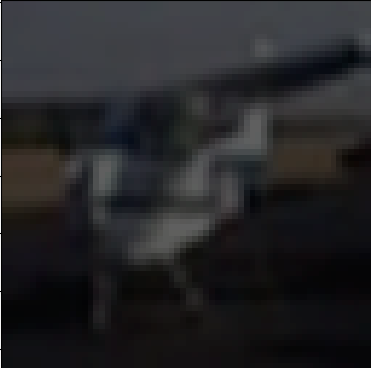
\includegraphics[width=0.35\textwidth]{I.png}}
\hspace{0.05\textwidth}
\subfigure{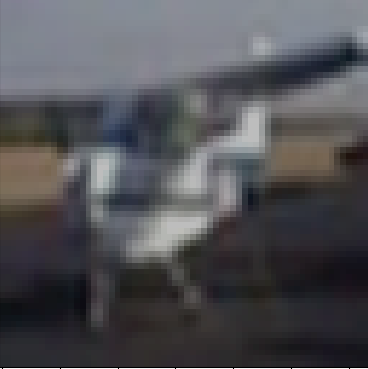
\includegraphics[width=0.35\textwidth]{I1.png}}
\end{figure}

\begin{figure}[H]
\subfigure{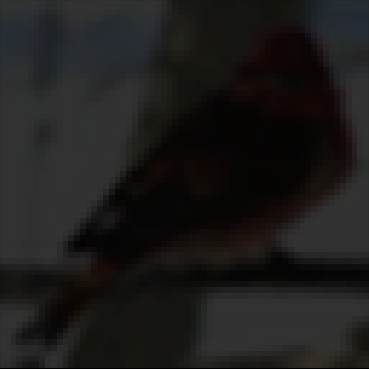
\includegraphics[width=0.35\textwidth]{I2.png}}
\hspace{0.05\textwidth}
\subfigure{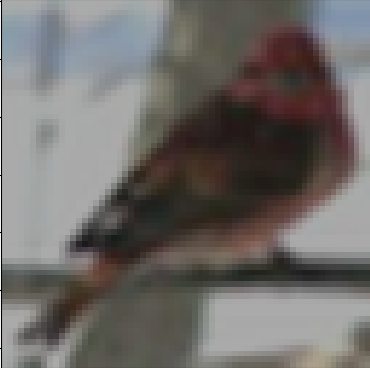
\includegraphics[width=0.35\textwidth]{I3.png}}
\end{figure}

\begin{figure}[H]
\subfigure{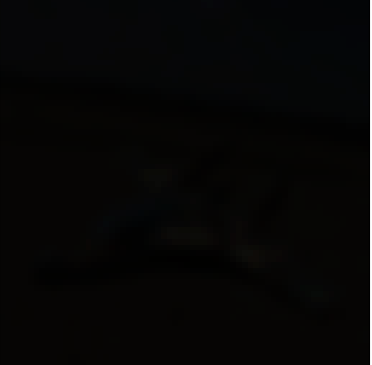
\includegraphics[width=0.35\textwidth]{I4.png}}
\hspace{0.05\textwidth}
\subfigure{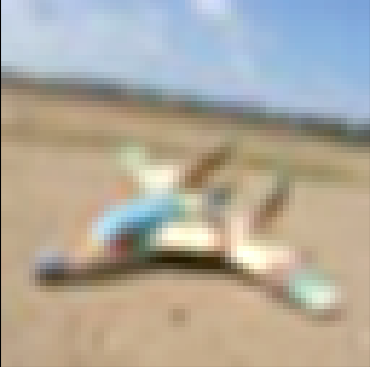
\includegraphics[width=0.35\textwidth]{I5.png}}
\end{figure}

\begin{figure}[H]
\subfigure{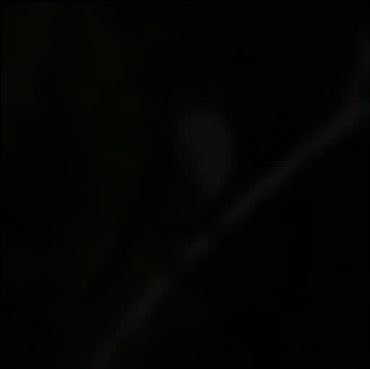
\includegraphics[width=0.35\textwidth]{I6.png}}
\hspace{0.05\textwidth}
\subfigure{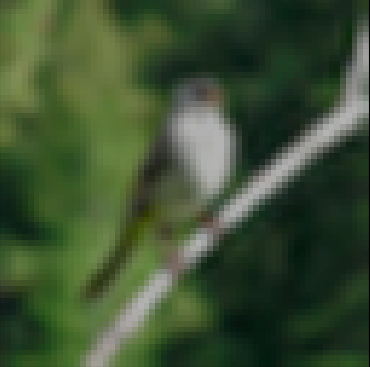
\includegraphics[width=0.35\textwidth]{I7.png}}
\end{figure}

\begin{figure}[H]
\subfigure{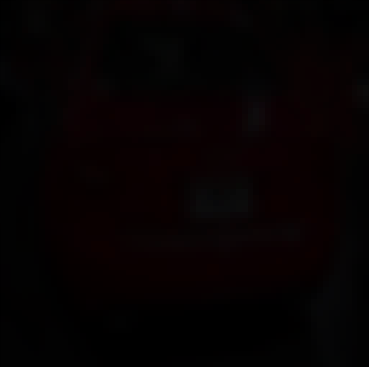
\includegraphics[width=0.35\textwidth]{I8.png}}
\hspace{0.05\textwidth}
\subfigure{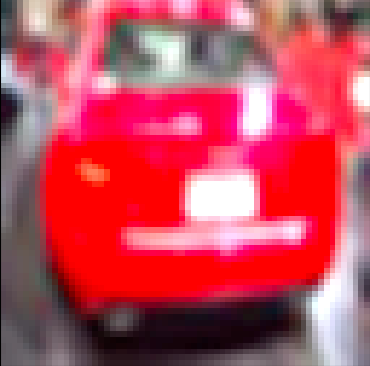
\includegraphics[width=0.35\textwidth]{I9.png}}
\end{figure}

\begin{figure}[H]
\subfigure{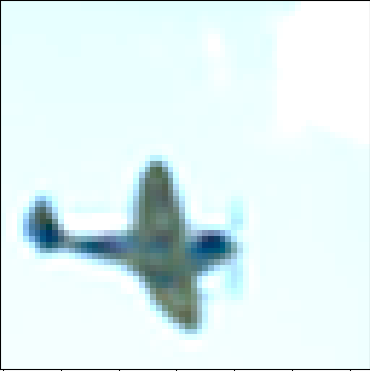
\includegraphics[width=0.35\textwidth]{I12.png}}
\hspace{0.05\textwidth}
\subfigure{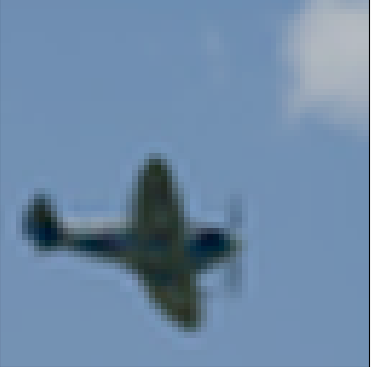
\includegraphics[width=0.35\textwidth]{I13.png}}
\end{figure}

\section{References}
$[1]$ Learning Photographic Global Tonal Adjustment with a Database of Input/Output Image Pairs \\
$[2]$ Personalized Exposure Control Using Adaptive Metering and Reinforcement Learning

%%%%%%%%%%%%%%%%%%%%%%%%%%%%%%%%%%%%%%%%%%%%%%%%%%%%%%%%%%%%%%%%%%%%%%%%%%%%%%%%%%%%%%%%%%%%%%%%%%%%%%%%%%%%%%%%%%%%%%
\end{document}
